% A simple graph with straight and bend arrows and loops
% Stefan Kottwitz
\documentclass{standalone}
\usepackage{tikz}
\usetikzlibrary{arrows}
\begin{document}
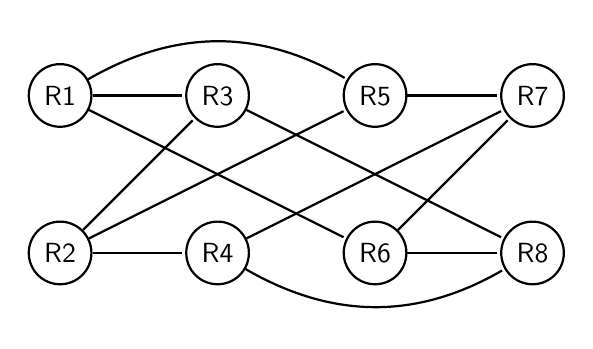
\begin{tikzpicture}[-,>=stealth',shorten >=1pt,auto,node distance=2cm,
  thick,main node/.style={circle,fill=white!15,draw,font=\sffamily}]

  \node[main node] (1) {R1};
  \node[main node] (2) [below of=1] {R2};
  \node[main node] (3) [right of=1] {R3};
  \node[main node] (4) [right of=2] {R4};
  \node[main node] (5) [right of=3] {R5};
  \node[main node] (6) [right of=4] {R6};
  \node[main node] (7) [right of=5] {R7};
  \node[main node] (8) [right of=6] {R8};
  
  \path[every node/.style={font=\sffamily\small}]
    (1) edge node [left] {} (3)
        edge [bend left] node[left] {} (5)
        edge [left] node [left] {} (6)
    (2) edge node [left] {} (3)
        edge [right] node[left] {} (4)
        edge [right] node [left] {} (5)
    (3) edge node [left] {} (8)
    (4) edge node [left] {} (7)
        edge [bend right] node[left] {} (8)
    (5) edge node [left] {} (7)
    (6) edge node [left] {} (7)
        edge [right] node[left] {} (8);
\end{tikzpicture}
\end{document}